% Chapter X

\chapter{Simulation of One Way Quantum Computation} % Chapter title

\label{ch:simul} % For referencing the chapter elsewhere, use \autoref{ch:name} 

For the next part of the project, a simulation was to be created that would allow for investigation of levels of fault tolerance for different logical qubits in the error correction scheme through Monte Carlo methods. The program would provide simulations of the single gate operations with randomised errors being introduced to the state vector of the system between the encoding and measurement steps. With these randomised errors and by comparing the outputs of the program with expected results, the fault tolerance of each set-up could be determined through repeated running of the program and collection of data. By then comparing the fault tolerance between various sizes of logical qubit in 'triangle' or 'pentagon' states etc, a correlation between fault tolerance and logical qubit size could be established to aid in choice of error correction scheme based on physical parameters of a system.


%----------------------------------------------------------------------------------------

\section{Set-up}

The first step of any simulation is, of course, to establish how the problem will be solved. In this regard, the simulation was first planned in pseudo code and the relevant components sketched out. This plan was somewhat ambitious as it encompassed a scheme for universal applications of one way quantum computation with the described error correction scheme. Though much of this plan was not completed, its contents are described in this section.

%------------------------------------------------

\subsection{Resources used}

For the simulation fortran 95 was chosen as an appropriate language due to it's scalability and ability to be broken up into modules. Details of the compilers, libraries and system used for simulation will be included in Appendix \ref{app:resources}.

Fortran 95 also contained standard functions to call for random numbers that were required for both measurement results and the addition of random errors as well as the ability to determine array sizes intrinsically, allowing for a tidier coding of subroutines.

%------------------------------------------------

\subsection{Subroutines}

A key requirement for the structure of any program was that it would be comprised of subroutines that handled the various steps of the operation of the modelled computer such that these subroutines could be easily rearranged in the main program to simulate any required topological structure. For example, the various single qubit operations required to satisfy universal computation in \citep{raussendorf_measurement-based_2003} can be simulated using the same physical system of a short chain of qubits but with different eigenbases for measurements. Hence in the simulation of a chain of spins the program was designed such that the required measurement operations could be read from a file allowing for any single qubit gate to be simulated with the same program.

Additionally, the two qubit CZ operation was written such that it could be performed between any two qubits in the state vector of the system, allowing it to be used in more complicated programs that would simulate the systems from the triangle states required for the basic implementation of the error correction code to the 8-qubit controlled phase gates.

As such every initialisation and measurement operation was set up to be self contained into one of three modules. The CZ operation module, the measurement module and an additional module that contained several linear algebra procedures required for the program to function. The modular structure also allowed for dynamic array allocation to occur at the top level of the program as array sizes could be passed to the various modules without need to include array sizes as extra arguments in calls to subroutines. This meant that all calls to internal subroutines were reasonably understandable and concise in the coding.

%------------------------------------------------

\subsection{Libraries}

As this program was primarily structured around matrices and linear algebra, extensive use of the BLAS external library as well as the LAPACK library \citep{lapack}. Not only would this make some calculation easier to code, but also meant that the program had some capacity for scalability onto parallel architectures given the structure of the routines in the library. Whenever possible BLAS was used in addition to intrinsic Fortran calls for dot products or matrix multiplication with preprocessor statements allowing the option of compiling without external libraries. However, as the program developed it became more dependant on these libraries and so is no longer functional without them.

%------------------------------------------------

\subsection{Precision}

As the program relied on numerical solutions to systems of linear equations, precision in variables was tantamount to functionality. As such IEEE 754 double precision \cite{_ieee_2008} was used in the program as standard in all real and complex variables, arrays and conversion functions. Because of this machine error was extremely low for all runs of the program, manifesting itself only in null values. While these null values may look untidy in current outputs for the program, they current provide a reasonable guarantee of numerical accuracy and can be easily cleared up in later versions through a rounding step before writing to file. 

However, this would mean that each double precision value in the state vectors of the subroutine or in operation matrices would be using 64 bits for each value stored. Hence the size of the system would quickly cause the memory usage to expand drastically. For a one dimensional chain of qubits, this is not a problem as qubits can be removed from the state vector after measurement, resulting in maximum memory usages of $~128 \times 2^{2}$ for the state vector. In the case of simulation of the quantum Fourier transform described in \citep{raussendorf_measurement-based_2003}, at least 20 qubits would be required, causing memory requirements of $~128 \times 2^{20}$ bits, which would be around 17 megabytes. While this is easily manageable for single qubits, incorporation of the triangle states as an error correction code would require around 18,000 petabytes, a value clearly infeasible for computation as even the top supercomputers have access to even one petabyte \citep{_top500_????} TOP 500 super computers. 

%----------------------------------------------------------------------------------------

\section{CZ Operation}

The first building block subroutine implemented into the program was a CZ operation subroutine. This subroutine would take a state vector and apply a CZ operation based on integer values of control and target bits. In this way, CZ operations could be achieved between any two qubits in the state vector, satisfying the requirements for initialisation of both measurement based single qubit gates and triangle states for error correction.

%------------------------------------------------

\subsection{Kronecker Product routine}

In order to generate the matrix describing the CZ operation between two qubits in the state vector, a subroutine was adapted from previous work \citep{children_spin_2013}, which was updated for Fortran 95's ability to intrinsically determine the size of an array. This subroutine for a Kronecker product was necessary to code as an equivalent was not found in the common external Fortran libraries. 

Using this subroutine CZ matrices were generated from $2 \times 2$ identity and Pauli-z matrices based on the the unitary operator \eqref{eq:u_final3}. 


\insertcode{"code_snippet/Code/cz_gen.f95"}{CZ generation main algorithm}

%------------------------------------------------

\subsection{Improvements}
As the CZ operation matrix is always diagonal, the subroutine could be easily improved to calculate and store the operation matrix as a one dimensional array. This would allow the use of a simpler Kronecker product routine designed only for vectors, but could also make calls to other subroutines unnecessary as the calculation of the operator would be reasonably trivial with a standard formula for generation that required only multiplication of negative numbers into the operator at the appropriate places.

Additionally, the array could be downscaled to integer values and then converted to double precision only when directly applied to the state vector, making savings in computation time and memory usage.

It would also be possible to generate CZ operators for the formation of triangle states similar to the unitary operator in \eqref{eq:logical3plus_u}. By generating these through a separate routine, the application of triangular CZ states shown in the equation \eqref{eq:add_triangle_cz} for the encoding of the logical cluster state, would be optimized further. This operation could even be generalised to satisfy pentagonal, heptagonal or any other alternative formation of logical qubits in the error correction scheme.

%----------------------------------------------------------------------------------------

\section{Other qubit operations}

One requirement for the modules of the program was that circuit model style operations would need to be performed in order to encode the error correction scheme into the system. 

%------------------------------------------------

\subsection{Pauli Z Operation}

While a Pauli Z operation was not coded into the program for single qubits, such a routine would be reasonably simple to implement using a simple modification of the CZ operation subroutine. Fundamentally the CZ operation includes two single qubit Z operations so by removing one of the nested loops the desired effect could be achieved. This subroutine could also be optimised as a diagonal matrix or as integer values in a similar way to the CZ operation, minimising memory usage and computational time.

%------------------------------------------------

\subsection{Hadamard Operation}

Similarly to the Pauli Z operation, the error correction scheme relies on the application of multiple Hadamard operations. Unlike the Z operation, this operator can be required to be applied to multiple qubits at the same time and as such requires a more complicated subroutine. Using the same Kronecker product subroutine it would be possible to form an operator that acts on an array of integers representing qubits to be operated upon. This way any possible error protection configuration could easily be handled by the same subroutine.

While this subroutine could not be held as a single dimensional array like the CZ and Z operations, it could still be stored as an integer, provided a real value be held as an additional variable to reflect the constant value multiplied by the matrix.

%------------------------------------------------

\subsection{Logical Operations}

In order to properly simulate the error correction protocols, the logical operators that are applied for both encoding and error correction need to be incorporated. These operators would be easily handled in the same way as the other operators described earlier as they can be seen to be components of the logical operators. As a result, the logical operator subroutines would operate at a higher level in the program, making use of the basic operators as resources. 

The key condition in designing a subroutine to function such that it can be used for larger logical qubits in order to compare the fault tolerance correlation between logical qubit sizes. This would be trivial to code however as it would just require the number of loops used to apply operations to all of the qubits comprising the logical qubits to be set in the argument of the subroutine rather than hard coded into the program. 


%----------------------------------------------------------------------------------------

\section{Measurement}

Obviously the most vital subroutine for the simulation of the operation of a measurement based quantum computation scheme is the act of measurement itself. Fundamentally, this subroutine must handle the functionality of any quantum algorithms whilst also supporting certain metaphysical principles and assumptions \citep{hagar_quantum_2011}. The program was designed to reflect the same metaphysical assumptions used in the algebraic model earlier and hence the model for measurement used earlier was also applied in the program.

%------------------------------------------------

\subsection{Random measurement in basis}

To reflect the random nature of measurement outcomes in each basis, the intrinsic random number generator in Fortran 95 was employed. This provided a random double precision number between 0 and 1 which was then rounded to the nearest integer value with the intrinsic function NINT(). This provided a simple way to deal with random measurement outcomes whilst also allowing for fixed outcomes in debugging as the default seed for the random number function is consistent, providing identical outcomes on each calling. Whilst seed generation for proper running of the program was explored, the time limited nature of programming meant that such features were never incorporated into the program at large, but it is likely that a seed generation library from the operating system would have been used or a custom one created based on system time.

The integer values representing the outcomes of the measurements were then written to file where they could be retrieved by the subroutine handling the feed-forward of measurement outcomes at the end of the program. 

%------------------------------------------------

\subsection{Pauli bases measurement}

In order to easily model CNOT, Hadamard and $\pi/2$ phase gates, a subroutine for measurement in the three Pauli bases which correspond to the eigenvectors of the $2 \times 2$ Pauli matrices was incorporated into the program. As these measurement bases were commonly used in almost all qubit gates it made sense to have them hard coded into the program instead of using a single generalised measurement routine 

\begin{equation}
\begin{array}{lclc}
  \sigma_{x+}=\displaystyle\frac{1}{\sqrt{2}}\!\!\!\!\! & \begin{pmatrix}{1}\\{1}\end{pmatrix}, & \sigma_{x-}=\displaystyle\frac{1}{\sqrt{2}}\!\!\!\!\! & \begin{pmatrix}{1}\\{-1}\end{pmatrix}, \\
  \sigma_{y+}=\displaystyle\frac{1}{\sqrt{2}}\!\!\!\!\! & \begin{pmatrix}{1}\\{i}\end{pmatrix}, & \sigma_{y-}=\displaystyle\frac{1}{\sqrt{2}}\!\!\!\!\! & \begin{pmatrix}{1}\\{-i}\end{pmatrix}, \\
  \sigma_{z+}=                                          & \begin{pmatrix}{1}\\{0}\end{pmatrix}, & \sigma_{z-}=                                          & \begin{pmatrix}{0}\\{1}\end{pmatrix}.
\end{array}
\end{equation}

In order to keep the programming concise, all three kinds of basis were included into the same subroutine which was controlled by a single character in the argument of the subroutine. This character would then be recorded in a file containing data about the measurements that could be used to calculate the final states in the feed forward subroutine. Currently however the program uses the phase directly, but this could be optimised in future iterations by hard coding the phase amounts of the Pauli bases into the feed forward routine. Unfortunately the Pauli Y and Pauli Z basis measurements do not work in the program when it comes to the final feed forward of measurement because of an error with the phase of the basis when it comes to feed forward of measurements to obtain the final state, so this change might even help alleviate that problem.

%------------------------------------------------

\subsection{Arbitrary measurement}

In addition the the Pauli bases measurements, a generalised measurement of arbitrary phase was also required for the program to implement the general rotation and z rotation single qubit gates. The subroutine for this process was very similar to the Pauli measurement subroutine aside from the inclusion of a variable measurement phase in the arguments of the subroutine and a general rotation vector replacing the eigenvectors of the Pauli bases. 

The subroutine, like the Pauli measurement subroutine, recorded the variable phase amount to a file so that it could be used in the feed forward subroutine as well as multiplying the result of the inner product of the measurement vector and the measured qubit state vector by the global state vector. Potentially this subroutine could be consolidated into the Pauli measurement subroutine through the use of the control character, likely with 'R' signifying a custom phase, but this is yet to be performed.

%------------------------------------------------

\subsection{Feed Forward}

The final necessary component of the measurement scheme consisted of a subroutine to feed forward measurement outcomes to recover the desired state at the end of the measurements. This subroutine performed the functionality of equation \eqref{eq:one_qbit_feed_forward} for the single qubit states. 

In order to achieve this result, the subroutine read the measurements performed over the course of the program in order and then applied \eqref{eq:one_qbit_feed_forward} for each measurement, leading to accurate results. 

The subroutine also has the functionality of being able to decompose larger state vectors in order to apply the feed forward results to specific qubits, but this is feature is currently unfinished.

%------------------------------------------------

\subsection{Multiple Outputs}

One of the weaknesses of the current subroutine to handle the feed forward of measurements is that it cannot deal with output state vectors consisting of multiple qubits simultaneously. For example, in the output state of the CNOT gate in equation \eqref{eq:CNOT_qbit_feed_forward}, a series of decoding operations are required to be performed on two qubits at once, which the subroutine would not be able to handle. 

Fortunately this is only a minor problem as the error correction scheme only requires a single output qubit and with sufficient time the subroutine could be updated to deal with such problems if deemed necessary.

%----------------------------------------------------------------------------------------

\section{Decomposition}

One of the critical elements to the functionality of the program was the ability to decompose the global state vector into individual qubit states in order for both the simulated measurement to be processed and the final state of the qubit to be determined. This required a reversing of the Kronecker product routine used to generate the state vector which presented a formidable challenge computationally.

While Kronecker products are not directly reversible, it is possible to determine a 'canonical' result for certain matrices. The principle behind this relies upon the relation between the Kronecker product and the vectorisation operator. Considering the vector $W$ which is a Kronecker product of two real vectors $U$ and $V$:

\begin{equation}
W = V \otimes U = vec(U V^{T})
\end{equation}

Vectorisation is a process which is easily reversed, so the vectors U and V can be recovered by decomposition of the resulting matrix. Note that for complex vectors $V^{T}$ becomes $V^{H}$ which represents the conjugate transpose of $V$.

\begin{equation}
U V^{T} = vec^{-1} (W)
\end{equation} 

Unfortunately, there are a wide range of possible decompositions, so this is where a canonical decomposition must be decided upon in order to progress further. 

%------------------------------------------------

\subsection{Rank decomposition}

The first subroutine developed to perform this decomposition was a simple rank 1 decomposition. It was originally thought that this would be sufficient in all cases as the Kronecker product of two vectors would always be rank one. However this was short-sighted as the application of the CZ operation modified the rank of the state vector, a phenomenon which seems to be representative of the entanglement induced in the system.

The algorithm worked by pulling the first non-zero column of the matrix formed from the inverse vectorisation of $W$ and normalising it. Then the algorithm divided each value of the first non-zero row by the new normalised values to obtain the other vector.

For a rank 1 state vector of pure such as $\ket{00}$ the algorithm was successful, but when encountering mixed states, the algorithm could not handle the input and returned null values. This was obviously unacceptable as the CZ operation will always make mixed states out of pure input states.

\insertcode{"code_snippet/Code/r1_decomp.f95"}{Rank decomposition algorithm}

%------------------------------------------------

\subsection{Single value decomposition}

As the rank decomposition was not a sufficient way to canonically decompose the matrix, the single value decomposition (SVD) was chosen as an alternative. As this was an $M \times N$ decomposition it would allow for particular qubits to be determined, compared to something like the eigen-decomposition which would only work with square matrices and thus be only able to break the state vector in half. 

Fortunately, unlike the rank decomposition there are plenty of available libraries for single value decomposition. For the simulation the double precision complex general decomposition routine zgesvd was chosen from the LAPACK library as it both complied with the established IEEE 754 precision standard and allowed for decomposition of a general matrix.

However, the SVD is a little more complicated than the rank decomposition as the matrix is broken into three parts. In the case of a complex matrix these consist of a diagonal matrix $\boldsymbol{\Sigma}$ of the singular values $\sigma_{i}$ of the matrix and two matrices $\mathbf{U}$ and $\mathbf{V}$ composed of rows and columns of vectors such that:

\begin{equation}
\mathbf{M} = \mathbf{U} \boldsymbol{\Sigma} \mathbf{V}^{H}
\end{equation}

When performing this decomposition in the program the resulting vectors $U$ and $V^{H}$ were assumed to be the summations of the rows or columns of matrices $\mathbf{U}$ and $\mathbf{V}$ respectively, while the $i$-th rows of $\mathbf{U}$ were multiplied by the corresponding single values $\sigma_{i}$.

The routine was tested with the application of a pauli X basis measurement on a pair of two qubits initialised in the $\ket{+}$ state before having the CZ operation applied. The resulting state vector of this initialisation was:

\begin{equation}
W =
\begin{pmatrix}
\frac{1}{2} \\
\frac{1}{2} \\
\frac{1}{2} \\
- \frac{1}{2} \\
\end{pmatrix}
\end{equation}

So when inverse vectorisation was applied this became:

\begin{equation}
\mathbf{M} =
\begin{pmatrix}
\frac{1}{2} &
\frac{1}{2} \\
\frac{1}{2} &
- \frac{1}{2} \\
\end{pmatrix}
\end{equation}

When entered into the subroutine the output was:

\begin{align}
\mathbf{U} &=
\begin{pmatrix}
-\frac{1}{\sqrt{2}} &
-\frac{1}{\sqrt{2}} \\
-\frac{1}{\sqrt{2}} &
\frac{1}{\sqrt{2}} \\
\end{pmatrix}
&
\boldsymbol{\Sigma} &=
\begin{pmatrix}
\frac{1}{\sqrt{2}} &
0 \\
0 &
\frac{1}{\sqrt{2}} \\
\end{pmatrix}
&
\mathbf{V}^{H} &=
\begin{pmatrix}
-1 &
0 \\
0 &
-1 \\
\end{pmatrix}
\end{align}

So the vectors $U$ and $V$ became:

\begin{align}
U =
\begin{pmatrix}
\frac{2}{\sqrt{2}} \\
0 \\
\end{pmatrix}
V =
\begin{pmatrix}
\frac{1}{\sqrt{2}} \\
\frac{1}{\sqrt{2}} \\
\end{pmatrix}
\end{align}

When the measurement in the Pauli X basis was applied, in case one:

\begin{multline}
\ket{+} \braket{+|U} \otimes \ket{V} \\
= \ket{+} (\frac{1}{\sqrt{2}}\frac{2}{\sqrt{2}} \braket{0|0}) \otimes \ket{V} \\
= \ket{+} \otimes \ket{V} \\
\end{multline}

Feeding the measurement result forward to determine the output state then gives:

\begin{equation}
e^{0} X^{0} H R_{0} \ket{V}
= H
\begin{pmatrix}
\frac{1}{\sqrt{2}} \\
\frac{1}{\sqrt{2}} \\
\end{pmatrix}
= \ket{0}
\end{equation}

Similarly for the other measurement outcome:

\begin{equation}
e^{0} X^{1} H R_{0} \ket{V}
=  X H
\begin{pmatrix}
\frac{1}{\sqrt{2}} \\
\frac{1}{\sqrt{2}} \\
\end{pmatrix}
= \ket{1}
\end{equation}

These outcomes match the expected outcomes for measurements of the qubit in the pauli X basis which is easily seen by looking measurement of the state expressed in the form described in equation \eqref{eq:2qubit_example}. In case 1:

\begin{equation}
\label{eq:m_outcome_1}
\bra{+} \frac{1}{\sqrt{2}} (\ket{+ 0} + \ket{- 1}) = \ket{0} = H \ket{+}
\end{equation}

And in case 2:

\begin{equation}
\label{eq:m_outcome_2}
\bra{-} \frac{1}{\sqrt{2}} (\ket{+ 0} + \ket{- 1}) = \ket{1} = XH \ket{+}
\end{equation}

Unfortunately the decomposition has not been tested for larger or more complex state vectors due to time constraints. However, it seems like there will be certain matrices which will throw up errors due to the multiplication of zero values or through the summation of rows and columns being zero, this could be fixed by performing multiple decompositions until a satisfactory decomposition for which zero values are minimised is achieved, but this would take extra computational resources and be mathematically untidy. In this regard, it seems that there must be a better way to reconstruct the vectors from the decomposition matrices but so far this remains unclear.


%----------------------------------------------------------------------------------------

\section{Error}

One of the crucial functionalities a completed program would be the ability to add randomised errors to a single or multiple qubits in a state vector of any size in order for the fault tolerance of each system to be analysed. Such a subroutine was only in its early stages in the program as it had not yet advanced to the stage of implementation of the error correction scheme necessary for the subroutine to be meaningful, but a clear plan had been drawn up as to how errors would be implemented numerically into the system. Ideally error would be induced between the CZ and measurement operations, as this would be consistent with the state vector that is resilient to errors in the error correction scheme, but error could be easily added to the state vector of the system at any time.

%------------------------------------------------

\subsection{Flip error}

Flip errors are reasonably easy to simulate in the state vector in any size as they can be effectively expressed as the application of a Pauli X operation to a qubit. In order to operate on a single qubit, or multiple, the Kronecker product subroutine would be employed to form operator matrices of appropriate size in a similar fashion to the way operators would be used to initialise the system with the error correction scheme. For example the operator operation applied to flip qubit $i$ in a state vector of $N$ qubits would be:

\begin{equation}
\mathbb{1}_{1} \otimes \mathbb{1}_{2} \otimes \dotsb \sigma_{X} \dotsb \otimes \mathbb{1}_{N}
\end{equation}

It is therefore clear that such an operator could easily be produced with nested loops of the Kronecker product subroutine, what remains unclear however is as which qubits the flips would be applied and at what rate. 

The simple way to decide which qubits to flip would be to have a universal error rate for bit flips and then include either Pauli operators or identity operators depending on whether a random number meets the threshold of the error rate. This would have the bonus effect of saving memory and calculation time compared to performing each flip individually as well as simplifying the programming of any subroutine handling errors.

The alternative to this would be to have separate error rates for each number of errors so that the number of errors are calculated and then assigned to random qubits in the following step. This would be particularly useful when testing whether the error correction scheme protects against particular numbers of phase flips, though would obviously cause a slight interest in computational requirements.

One advantage to only modelling phase flips however is that any operator matrix can be stored in integer form and only converted to double precision when multiplying out with the state vector. This would save large amounts of memory compared to a phase error matrix which would require double precision storage and thus have memory requirements equal to the square of the memory requirements of the state vector.

%------------------------------------------------

\subsection{Phase error}

Similarly to the flip error, phase errors can be simulated through the inclusion of a phase operation on a qubit in the state vector. However, the phase of the error present provides another variable for the model as phase errors are obviously continuous variables rather than the discrete flip errors. Hence not only would a random number of qubits need to be exposed to the error, the exact value of the error would also need to be determined. While this could be done with a fixed error, something like a Gaussian distribution would work reasonably well for modelling. Indeed, if a a Gaussian distribution with a particularly high standard deviation were used, Phase errors could be applied to every qubit, reducing the number of steps in calculation of the operator. 

%----------------------------------------------------------------------------------------

\section{Data Analysis}

Another key component for the program is the ability to analyse cohesive and accurate output data. This puts requirements on the format of output data as well as the method of storage. For the program in its current form, data is output formally from the fidelity function, the value of the state vectors is printed directly to standard output, which was typically piped into a separate file.

%------------------------------------------------

\subsection{Fidelity}

In order to determine if the output state and expected output state correspond to one another, a fidelity subroutine was also included in the program. Like the Kronecker product subroutine, this subroutine was adapted from earlier work and simply performed the basic calculation:

\begin{equation}
\text{Fidelity} = |\braket{\text{Expected State}|\text{Final State}}|^{2}
\end{equation}

Like the other subroutines in the program, this calculation could be performed with or without the BLAS library's complex double precision dot product routine (ZDOTU) and as such has potential for scalability into parallel processing.

%------------------------------------------------

\subsection{Bulk data}

The ideal end result for a complete program would involve a large data set of fidelity data from multiple runs of the program. As a result some changes would have to be made so that fidelity data was instead appended to the file. Once this had been done, a scatter plot between the number of gates performed on the data and the fidelity of the result would be plotted for each size of logical qubit. 

This data would then be fitted to a curve using whatever method best worked for the output in order to establish the correlation between the two axes depending on the fixed error rate from the program. This would hopefully lead to a better understanding of the way in which fault tolerance was affected by the size of logical qubits for this measurement scheme.

%----------------------------------------------------------------------------------------

\section{Error Correction Scheme}

The final part of the program is the incorporation of the error correction scheme. This involves two main subroutines, the encoding subroutine and the detection/correction subroutine. 

%------------------------------------------------

\subsection{Encoding}

The encoding subroutines main function would be reflective rotational operation combined with the method for forming logical CZ operators described in section \ref{sec:entag_3_qb}. This would be challenging to perform and would require a great deal of coding in order for the operations to be scalable to any size logical qubit.

%------------------------------------------------

\subsection{Correction}

Correction, in comparison, would be a little easier to implement as the measurement routine currently in use for the program could be recycled for the bulk of the functionality. The main challenge would then be the conditional statements to implement the scheme and apply the appropriate logical operations depending upon the measurement outcomes. There would also need to be a small decoding step also, but this could be adapted from the encoding step which would need to be implemented first for correction to be possible in the first place.

%----------------------------------------------------------------------------------------

\section{Other structures}

In addition to testing the error correction scheme on single qubit gates, there are some other gates and set-ups that would be both interesting and useful to simulate with the program. These structures are of interest in particular as they represent the key building blocks of common quantum algorithms.

%------------------------------------------------
\subsection{Controlled not gate}

The first interesting structure that would make a good extension to the program would be a controlled not gate, though implementation would require the problems with the feed forward subroutine being unable to deal with multiple qubit state vectors to be rectified.

Obviously one of the advantages of demonstrating that this structure can be fault tolerant is that, when combined with the single qubit gates, forms a universal set of quantum gates. This means that such a demonstration would be necessary to prove the validity of the error correction scheme as universal.

Unlike the single qubit gates, it would not be possible to perform this operation repetitively without the introduction of new control qubits. While this is not too difficult a problem to overcome, it would make comparison of final results with expected outcomes more challenging as the expected outcomes would require far more calculation than repetitive use of a $\pi / 2$ gate, for example.

%------------------------------------------------

\subsection{Controlled phase gate}

A very interesting structure for simulation by the program, would be a controlled phase gate. This structure is interesting both because not only can it be represented without the decompositions into CNOTs and rotations required for the circuit model, but it is also a crucial building block for the Quantum Fourier transform algorithm \citep{raussendorf_measurement-based_2003}. 

\begin{figure}
\centering
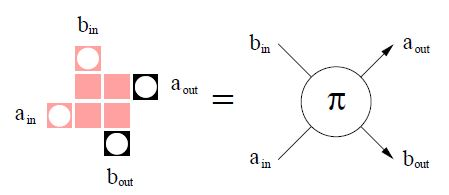
\includegraphics[scale=0.9]{gfx/phasegate.JPG}
\caption{Controlled phase gate structure and functionality
 \citep{raussendorf_measurement-based_2003}}
\label{fig:phase_gate}
\end{figure}

This structure, show in figure \ref{fig:phase_gate}, consists of 8 qubits in a spiral pattern with measurements performed on the central square, far simpler than the chain of gates required in the circuit model. However, like the CNOT gate, implementation of a measurement feed forward subroutine that could handle multiple outputs would be required. Implementation of this structure into the model with the error correction code would be also quite interesting given the entanglement of four qubits simultaneously, which would present an interesting programming challenge.

%------------------------------------------------

\subsection{Quantum Fourier transform}

If the program can simulate controlled phase gate, the Fourier transform is also possible with sufficient computational resources. As shown in 'Measurement-based quantum computation on cluster states', this structure can be constructed from six controlled phase gates and three Hadamard gates \citep{raussendorf_measurement-based_2003}. This particular structure is of great interest as it forms a crucial part of Shor's algorithm, making implementation highly desirable. However, memory usage of implementation for this structure in conjunction with an error correction scheme would be problematic given its high requirements on the number of qubits that are simultaneously active. It is possible that the components of the structure could be broken down in order to minimise the required computational resources through the inclusion of unitary gates between controlled phase gates and the simulation of each phase gate individually, but as yet this seems difficult to envision.

\begin{figure}
\centering
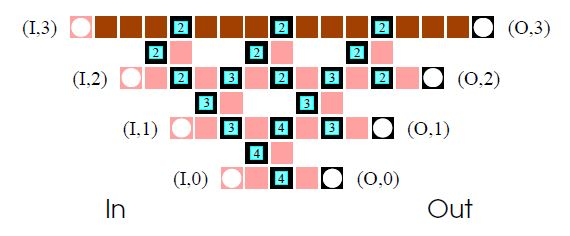
\includegraphics[scale=0.75]{gfx/qft.JPG}
\caption{Quantum Fourier transform schema \citep{raussendorf_measurement-based_2003}}
\end{figure}